\documentclass[tikz]{standalone}
\usetikzlibrary{automata,positioning}
\begin{document}

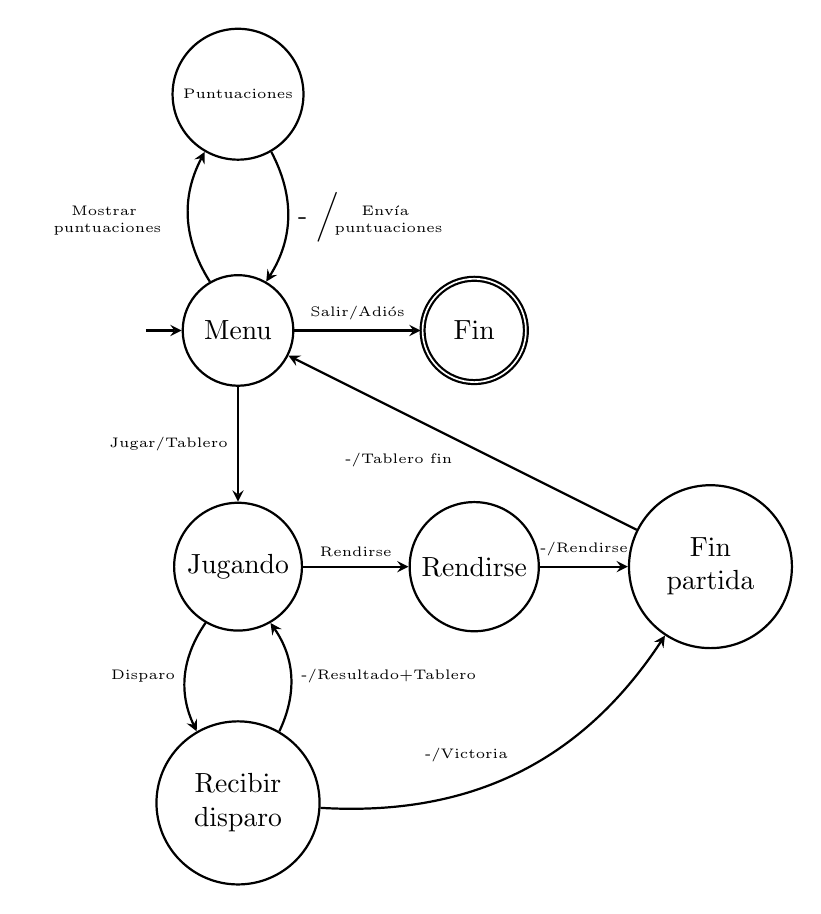
\begin{tikzpicture}[>=stealth,node distance=3cm,on grid,auto, thick, initial text=]
  \node[state, initial] (menu) {~Menu~~};
  \node[state] (jugando) [below=of menu] {Jugando};
  \node[state] (puntuaciones) [above=of menu] {\tiny Puntuaciones};
  \node[state] (recibir_disparo) [below=of jugando] {\begin{tabular}{c} Recibir \\ disparo \end{tabular}};
  \node[state] (rendirse) [right=of jugando] {Rendirse};
  \node[state] (fin_partida) [right=of rendirse] {\begin{tabular}{c} Fin \\ partida \end{tabular}};
  \node[state, accepting] (end) [right=of menu] {~~Fin~~~};
  
  \path[->]  (menu) edge [bend left] node {\begin{tabular}{c} \tiny Mostrar \vspace{-2mm} \\ \tiny puntuaciones \end{tabular}} (puntuaciones)
  (puntuaciones) edge [bend left] node {- \Big/ \hspace{-5mm} \begin{tabular}{c} \tiny Envía \vspace{-2mm} \\ \tiny puntuaciones \end{tabular}} (menu)
  (menu) edge node [left] {\tiny Jugar/Tablero} (jugando)
  (menu) edge node {\tiny Salir/Adiós} (end)
  
  (jugando) edge node {\tiny Rendirse} (rendirse)
  (jugando) edge [bend right] node [left] {\tiny Disparo} (recibir_disparo)
  
  (recibir_disparo) edge [bend right] node [right] {\tiny -/Resultado+Tablero} (jugando)
  (recibir_disparo) edge [bend right] node {\tiny -/Victoria} (fin_partida)

  (rendirse) edge node {\tiny -/Rendirse} (fin_partida)
  (fin_partida) edge node {\tiny -/Tablero fin} (menu);
\end{tikzpicture}
\end{document}
